\documentclass{article}
% General document formatting
\usepackage[margin=0.7in]{geometry}
\usepackage[parfill]{parskip}
\usepackage[utf8]{inputenc}
\usepackage{graphicx}
\usepackage{enumitem}

% Related to math
\usepackage{amsmath,amssymb,amsfonts,amsthm,bm}

% \newcommand{\ddx}[1][f{(x)}]{\frac{d}{dx}\left(#1\right)}
\newcommand{\xhat}{\hat{\textbf{x}}}
\newcommand{\yhat}{\hat{\textbf{y}}}
\newcommand{\zhat}{\hat{\textbf{z}}}
\newcommand{\del}{\vec{\nabla}}

\title{Physics 408\\[0.5em]
	Build Your Own Problems\\
}
\author{Max Varverakis}

\begin{document}
\maketitle

\section*{Griffiths 1.34}
This problem is a modification of Griffiths 1.34. The original problem asks us to verify Stokes' theorem for the vector function $\vec{v} = (xy)\xhat + (2yz)\yhat + (3zx)\zhat$ using the triangular surface made by connecting vertices $(0,0,0)$, $(0,2,0)$, and $(0,0,2)$. In the original problem, the integrals are shown to be
\begin{equation}
	\int_{S}(\del\times\vec{v})\cdot d\vec{a} = \oint_{C}\vec{v}\cdot d\vec{l} = -\frac{8}{3}.
\end{equation}

\subsection*{Adaptation}
I want to modify the surface that we use to test Stokes' theorem. In particular, I want to connect the points $(0,2,0)$ and $(0,0,2)$ by a circular arc.

\subsection*{Solution}
The figure below depicts the modified surface. Each path segment is labeled with a number.
\begin{figure}[htpb]
	\centering
	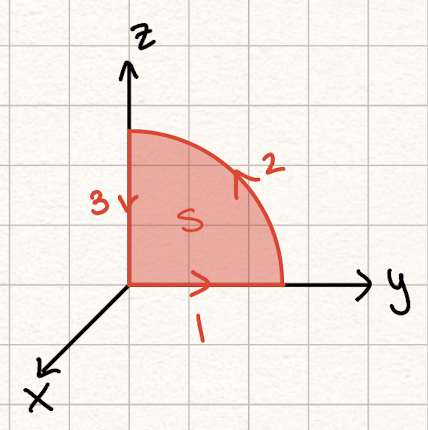
\includegraphics[width = .25\textwidth]{1.34.png}
\caption{Modified surface for Stokes' theorem.}
\end{figure}

First, let's calculate the surface integral. We have the following:
\begin{itemize}
	\item $d\vec{a} = dydz\xhat$ as by the right-hand rule convention.
	\item $\del\times\vec{v} = (-2y)\xhat + (-3z)\yhat + (-x)\zhat = (-2y)\xhat + (-3z)\yhat + 0\cdot\zhat$ since $x=0$ for this surface. Therefore, $(\del\times\vec{v})\cdot d\vec{a} = (-2y)dydz$.
	\item Note that the upper integration bound for $y$ is $\sqrt{4-z^2}$ since path 2 is an arc from a circle of radius $2$ centered at $(0,0,0)$ with corresponding equation $y^2 + z^2 = 4$.
\end{itemize}
The surface integral is then
\begin{equation}
	\int_S(\del\times\vec{v})\cdot d\vec{a} = \int_0^2dz\int_0^{\sqrt{4-z^2}}(-2y)dy = -\frac{16}{3}.
	% \int_0^1dz\int_0^{\sqrt{4-z^2}}(-2y)dy = -\int_0^1 y^2\Big|_0^{\sqrt{4-z^2}} dz
\end{equation}

Next, we calculate the integral over the boundary of the surface. Since $d\vec{l} = \xhat dx + \yhat dy + \zhat dz$, it follows that
\begin{equation}
	\vec{v}\cdot d\vec{l} = (xy)dx + (2yz)dy + (3zx)dz = 2yz dy
\end{equation}
with the simplification due to $x=0$.

Let's calculate the line integral over each path segment:
\begin{enumerate}
	\item For path $(1)$, $x=z=dx=dz=0$ where $y:0\to2$. Plugging in, this gives $\vec{v}\cdot d\vec{l} = 0$. Clearly, this path segment does not contribute to the line integral. In other words, 
	\begin{equation}
		\int\vec{v}\cdot d\vec{l} = 0.
	\end{equation}
	
	\item For path $(2)$, $x=dx=0$. We parameterize $y$ in terms of $z$ by $y = \sqrt{4-z^2}$ where $z:0\to2$. Thus, $dy = -\frac{z}{\sqrt{4-z^2}}dz$. Now, in terms of our parameterization, we can rewrite $\vec{v}\cdot d\vec{l} = 2yzdy = -2z^2dz$. Therefore, the line integral over path $(2)$ is
	\begin{equation}
		\int\vec{v}\cdot d\vec{l} = -2\int_0^2z^2dz = -\frac{16}{3}.
	\end{equation}

	\item Lastly, we have to integrate over path $(3)$. We have $x=y=dx=dy=0$ and $z:2\to0$. Thus, $\vec{v}\cdot d\vec{l} = 0$ after plugging in for $y$ and $dy$. Similar to path $(1)$, $\vec{v}\cdot d\vec{l} = 0 \implies \int\vec{v}\cdot d\vec{l} = 0$.
\end{enumerate}
To find the integral around the closed loop of $(1)\to(2)\to(3)$, we add the line integrals over each path segment to obtain
\begin{equation}
	\oint\vec{v}\cdot d\vec{l} = 0 - \frac{16}{3} + 0 = -\frac{16}{3}.
\end{equation}

Both the surface and line integrals are equal to $-\frac{16}{3}$, so Stokes' theorem is verified for this modified surface!

\end{document}